\chapter{Implementaciones}
\label{chap:libs}

\section{Librerías}

Hay varias implementaciones de criptografía homomórfica, y varias soluciones por cada una de las generaciones. Aunque la mayoría de las implementaciones están escritas para \verb|C/C++/C#|, recientemente han ido apareciendo algunas nuevas que buscan, principalmente, adaptar los esquemas de cifrado a otros lenguajes. Aunque esto es una buena noticia, nosotros nos centraremos en las "clásicas" evaluadas por el consorcio de estandarización:

\begin{itemize}
    \item Segunda generación
    \begin{itemize}
        \item HELib
        \item Microsoft SEAL
        \item PALISADE
        \item HeaAn
        \item LoL
        \item NFLlib
    \end{itemize}
    \item Tercera generación
    \begin{itemize}
        \item TFHE
        \item FHEW
        \item cuHE
    \end{itemize}
\end{itemize}

Para nuestro trabajo utilizaremos las librerías Microsoft SEAL (como representante de la segunda generación de criptografía homomórfica) y TFHE (como representante de la tercera). Para la segunda generación habría sido también una muy buena opción utilizar PALISADE, pero la documentación es mucho menor, y no incluye el esquema CKKS (necesario para trabajar con números reales).

\section{Microsoft SEAL}
\label{tag:msfseal}

Esta librería de código abierto desarrollada por Microsoft (\textit{SEAL} de ahora en adelante) busca ofrecer una opción asequible para los desarrolladores de implementar soluciones con criptografía homomórfica.

Es muy fácil de instalar, no tiene dependencias externas, y está diseñada para ser construida en cualquier entorno con \verb|cmake|.

Cuenta con dos esquemas de cifrado de segunda generación (BGV y CKKS) y dentro de su código fuente se incluyen varios ejemplos que muestran cómo se opera con ella. En estos ejemplos, ordenados para conocer las distintas herramientas, muestran todo lo necesario para empezar a trabajar.

A la hora de implementar una idea en SEAL, hay dos aspectos clave a tener en cuenta:

\begin{enumerate}
  \item Elegir el esquema de cifrado que nos permita codificar todo correctamente
  \item Estudiar si la operación realmente es realizable con estos esquemas (recordemos que SHE tiene una cota de cómputo)
\end{enumerate}

Además, hay que ser consciente de que bajo determinados usos, puede ser insegura. Por ejemplo, no se debe permitir el descifrado desde un entorno no controlado (no es CCA seguro (\cite{peng_danger_2019})).

\subsection{API}

La API para operar con SEAL está codificada en los siguientes elementos:

\begin{itemize}

  \item EncryptionParameters
  
  Parámetros descriptivos de los elementos criptográficos

  \item SEALContext

  Contexto del texto cifrado (cambia a medida que se opera)

  \item Claves

  \begin{itemize}

    \item SecretKey

    Clave secreta para descifrar los datos

    \item PublicKey

    Clave pública para cifrar los datos

    \item RelinKeys

    Claves públicas para realinearizar los datos y reducir el nivel de error acumulado tras operar

    \item GaloisKeys

    Claves públicas para trabajar con rotaciones en los vectores cifrados (en nuestro ejemplo no las usamos)

  \end{itemize}

  \item Encryptor, Decryptor

  Sistemas para cifrar y descifrar los datos

  \item Evaluator

  Es el componente que realiza las operaciones sobre los datos cifrados

  \item Encoder

  Encargado de codificar los datos en función del esquema que se desee utilizar

\end{itemize}

A continuación explicaremos más detalladamente el funcionamiento de los componentes más complejos.

\subsection{EncryptionParameters}

Los parámetros criptográficos dependerán del esquema con el que se quiere trabajar.

\subsubsection{BFV}

BFV es el esquema "básico" de SEAL. Permite trabajar con números enteros, y operar con ellos hasta que se alcanza el límite máximo de error. En BFV, este límite se podría conceptualizar como un cubo de fichas que se gastan cada vez que se opera.

Hay algunas operaciones que son casi gratuitas (la suma y la resta), y la multiplicación es muy costosa. Una vez se vacía este cubo (codificado en el parámetro \verb|noise_budget|), nuestro cifrado quedará corrupto y no se puede recuperar el texto.

Además de \verb|noise_budget|, hay tres parámetros configurables que guardan una estrecha relación:

\begin{itemize}
    \item \verb|poly_modulus_degree|
    
    Determina el módulo del polinomio usado para realizar las operaciones criptográficas (recordemos que implementa LWE sobre un anillo de polinomios, ver \ref{tag:bfv}). Se expresará como una potencia de 2 que cuanto más grande sea, más operaciones permitirá hacer, pero serán más lentas.
    
    \item \verb|coeff_modulus|
    
    Es un vector de números primos que determina el módulo del texto cifrado. A mayor módulo, mayor será el \verb|noise_budget|. Cuando decíamos que a mayor \verb|poly_modulus_degree|, podíamos hacer más operaciones, era porque el número de bits de \verb|coeff_modulus| está acotado por el de \verb|poly_modulus_degree| de la forma indicada en la figura \ref{table:poly_vs_coeff_modulus}
    
    \begin{table}
        \centering
        \begin{tabular}{  c  c  }
        \verb|poly_modulus_degree|  & Número de bits de \verb|coeff_modulus| \\
        \hline \hline \\
        1024  & 27  \\
        2048  & 54  \\
        4096  & 109 \\
        8192  & 218 \\
        16384 & 438 \\
        32768 & 881
        \end{tabular}
        \caption{Relación \textit{poly\_modulus\_degree}/\textit{coeff\_modulus\_degree}}
        \label{table:poly_vs_coeff_modulus}

    \end{table}
    
    \item \verb|plain_modulus|
    
    Modulo del texto plano. El consumo de \verb|noise_budget| se produce de forma logarítmica en base al tamaño de \verb|plain_modulus|, por lo que cuanto más pequeño es, más operaciones podremos realizar. También debe ser menor que \verb|poly_modulus_degree|.
\end{itemize}{}

\subsubsection{CKKS}

En la implementación del esquema CKKS podremos trabajar con número decimales, pero tendremos que realizar algunas gestiones adicionales a las de BGV para evitar que se pierda la integridad de nuestros cálculos.

Comparte con BGV tanto \verb|poly_modulus_degree| como \verb|coeff_modulus|, pero desaparece el elemento \verb|plain_modulus| (la integridad del texto cifrado ya no se evaluará con el \verb|noise_budget|), y los valores elegidos para \verb|coeff_modulus| tendrán otras implicaciones.

Aparece un elemento nuevo: la escala. De forma análoga a la que hemos implementado en la maqueta de THFE (ya lo veremos en el capítulo \ref{chap:poc}) para codificar los números decimales se aplica una escala (se multiplican por un valor muy alto, potencia de 2) y se tratan como número enteros.

Esta escala aumentará drásticamente cada vez que se multipliquen dos elementos. Siendo $N$ el tamaño del primer factor, y $M$ el del segundo, el resultado del producto tendrá como tamaño $M+N-1$. Para evitar que el número desborde su tamaño máximo, tras un producto puede reducirse la escala. La operación de reescalado implementada en SEAL trunca el valor del texto cifrado tantos bits como tenga el último elemento del vector \verb|coeff_modulus|, y elimina este elemento (cambiando el contexto de cifrado). De esta forma, siendo $P$ el tamaño del elemento eliminado de \verb|coeff_modulus| el texto cifrado pasaría a tener un tamaño $(M+N-1)/P$. Una vez se terminan los elementos de \verb|coeff_modulus| no se puede seguir operando, y se debe conservar siempre uno para poder realizar la operación de descifrado.

Para poder reescalar sin problemas se debe elegir una escala inicial menor que el número expresado por el último valor de \verb|coeff_modulus| (cuando \verb|coeff_modulus| está integro). Además, el primer valor de la cadena (el que se utilizará cuando se vaya a descifrar), debe ser mayor que el resto para poder tener cierta precisión: si este valor es 60, y el segundo (el que se utiliza al realizar la última operación) es 40, tendremos 20 bits de precisión ($60 - 40$) para los decimales al retirar la escala.

A continuación veremos en qué consisten exactamente el contexto y la cadena de la que hablamos.

\subsection{SEALContext, niveles de error y realinearización}

\verb|SEALContext| (lo que llamamos contexto, o contexto criptográfico) es la clase en la que se codifican las propiedades del texto cifrado, desde el esquema utilizado a los distintos parámetros de cifrado. La creación del \verb|SEALContext| genera una estructura similar a una cadena que guardará el estado de \verb|coeff_modulus|. De esta forma, podremos mantener la integridad al operar entre distintos textos cifrados símplemente verificando que esta cadena es igual.

Inicialmente, la cadena se inicializa con la información de \verb|coeff_modulus|, y va cambiando a medida que, por ejemplo, se aplican operaciones de reescalado. La cadena es una lista enlazada de los \verb|SEALContext| en cada momento de operación:

\begin{listing}[ht]
    \begin{minted}{console}
         special prime +---------+
                                 |
                                 v
coeff_modulus: { 50, 30, 30, 50, 50 }  +---+  Level 4
                                          |
                                          |
   coeff_modulus: { 50, 30, 30, 50 }  +---+  Level 3
                                          |
                                          |
       coeff_modulus: { 50, 30, 30 }  +---+  Level 2
                                          |
                                          |
           coeff_modulus: { 50, 30 }  +---+  Level 1
                                          |
                                          |
               coeff_modulus: { 50 }  +---+  Level 0
    \end{minted}
    \caption{Cadena de SEALContext (documentación de SEAL)}
    \label{fig:seal_levels}
\end{listing}

Se puede descender, pero nunca ascender. Cuanto más abajo, más rápidos son los cálculos, pero menos cálculos se pueden hacer. En ocasiones, debido al tamaño del texto plano, descender no tendrá consecuencias en cuanto al nivel de error, por lo que se podrá hacer para tener mayor eficiencia. En otros, será una condición indispensable para poder seguir operando. Es por esto que, cumpliendo los requisitos sobre el tamaño de \verb|coeff_modulus| con respecto a \verb|poly_modulus_degree|, y siguiendo las pautas que hemos comentado con respecto al primer y último elemento de la cadena, es recomendable que elijamos el mayor número de elementos intermedios posible.

Mientras que en BGV este contexto no tiene mucha importancia (más allá de la eficiencia) en CKKS la cosa cambia. Cuando se reescala en CKKS, se está eliminando al mismo tiempo parte de esta cadena. Por lo tanto, hay que tener en cuenta que si se ha reescalado, y se ha cambiado el contexto de cifrado de un elemento, tendremos que ajustar el contexto del resto de elementos que queramos operar con él (para que estén en la misma escala y usen los mismos parámetros criptográficos), ya sea reescalando (cuando sea necesario) o haciendo al elemento "descender" en la cadena.

Otra forma de reducir la velocidad a la que aumenta el nivel de error sin perder profundidad computacional (capacidad para realizar más operaciones) es la realinearización. Como hemos visto anteriormente, a medida que se opera, el error aumenta. La suma es casi gratuita, pero con el producto de dos elementos de tamaño $M$ y $N$, teniendo el resultado tamaño $M+N-1$, el error aumenta considerablemente. Interpretaremos este tamaño como el grado polinómico del elemento. La realinearización es una operación que permite, utilizando unas claves especiales (claves de realinearización), reducir el tamaño tras una multiplicación, reduciendo así el consumo de \verb|noise_budget| en las siguientes operaciones. Tiene un coste computacional alto en comparación con el resto de operaciones, pero permite operar de forma más eficiente, y que el elemento no crezca hasta "romperse" (o crezca de una forma más lenta).

\subsection{Encoders}

SEAL ofrece tres sistemas para codificar los datos con los que se va a trabajar:
\begin{itemize}
    \item \verb|IntegerEncoder| (para BFV)

    Codifica el número descomponiendolo en una sucesión de exponenciaciones para poder trabajar con sus subelementos de forma independiente.

    \item \verb|BatchEncoder| (para BFV)

    Crea una matriz $2 \times (N/2)$ con N el número de elementos codificables. Estos elementos son conocidos como \textit{slots}, y su número es igual a \verb|poly_modulus_degree|. En cada \textit{slot} se almacena un número en base modular $\mathbb{Z}_{plain\_modulus}$. Si se codifica un vector, se introducirá tal cual, y si sólo se codifica un valor, se llenarán todas las posiciones de la matriz con ese valor.

    \begin{gather}
      a =
      \begin{pmatrix}
        a & a & \hdots & a \\
        a & a & \hdots & a
      \end{pmatrix} &
      \begin{pmatrix}
        c_1 & c_2 & c_3
      \end{pmatrix}
      =
      \begin{pmatrix}
        c_1 & c_2   & c_3   & 0     & \hdots & 0 \\
        0   & 0     & 0     & 0     & \hdots & 0
      \end{pmatrix}
    \end{gather}

    \item \verb|CCKSEncoder|

    Funciona de forma similar al \verb|BatchEncoder|, pero tiene la mitad de posiciones con respecto al mismo \verb|poly_modulus_degree|.
\end{itemize}{}

\subsection{Trabajo con vectores}

Tanto \verb|BatchEncoder| como \verb|CKKSEncoder|, interpretan todos los datos como vectores. Una de las cosas más interesantes de esta forma de codificar los datos, es que se pueden rotar las columnas y las filas. Para ello será necesario el empleo de unas claves especiales llamadas \textit{Galois Keys}. La rotación es cíclica, es decir, cuando se rota una posición a la izquierda el primer valor pasa a la última posición.

\begin{itemize}
    \item Rotando filas
    
    % TODO GALOIS!!!
    
    \begin{gather}
        \begin{bmatrix}
            b_{11}  & b_{12}  & \hdots    & b_{1n} \\
            b_{21}  & b_{22}  & \hdots    & b_{2n}
        \end{bmatrix}
        \rightarrow
        \begin{bmatrix}
            b_{12}  & \hdots    & b_{1n}    & b_{11} \\
            b_{22}  & \hdots    & b_{2n}    & b_{21}
        \end{bmatrix}
    \end{gather}
    
    \item Rotando columnas 
    
    \begin{gather}
        \begin{bmatrix}
            b_{11}  & b_{12}  & \hdots    & b_{1n} \\
            b_{21}  & b_{22}  & \hdots    & b_{2n}
        \end{bmatrix}
        \rightarrow
        \begin{bmatrix}
            b_{21}  & b_{22}  & \hdots    & b_{2n} \\
            b_{11}  & b_{12}  & \hdots    & b_{1n} 
        \end{bmatrix}
    \end{gather}
    
\end{itemize}
%
%     [  0,  1,  2,  3,  0, ...,  0,  0,  0,  0,  0 ]
%     [  4,  5,  6,  7,  0, ...,  0,  0,  0,  0,  0 ]
%
% Line  60 --> Encode and encrypt.
%     + Noise budget in fresh encryption: 134 bits
%
% Line  78 --> Rotate rows 3 steps left.
%     + Noise budget after rotation: 134 bits
%     + Decrypt and decode ...... Correct.
%
%     [  3,  0,  0,  0,  0, ...,  0,  0,  0,  1,  2 ]
%
%     [  7,  0,  0,  0,  0, ...,  0,  0,  4,  5,  6 ]
%
% Line  92 --> Rotate columns.
%     + Noise budget after rotation: 134 bits
%     + Decrypt and decode ...... Correct.
%
%     [  7,  0,  0,  0,  0, ...,  0,  0,  4,  5,  6 ]
%     [  3,  0,  0,  0,  0, ...,  0,  0,  0,  1,  2 ]

Por otro lado, las operaciones aritméticas se realizan entre los valores de cada posición uno a uno, no como una operación entre matrices. Por ejemplo, el producto sería:

\begin{gather}
    \begin{bmatrix}
        a_{11}  & \hdots    & a_{1n} \\
        a_{21}  & \hdots    & a_{2n}
    \end{bmatrix}
    *
    \begin{bmatrix}
        b_{11}  & \hdots    & b_{1n} \\
        b_{21}  & \hdots    & b_{2n}
    \end{bmatrix} 
    =
    \begin{bmatrix}
        (a_{11} * b_{11})    & \hdots    & (a_{1n} * b_{1n}) \\
        (a_{21} * b_{21})    & \hdots    & (a_{2n} * b_{2n})
    \end{bmatrix}
\end{gather}



\subsection{Evaluator}

Por último, tras conocer todo lo que se puede hacer con SEAL, veremos cómo hacerlo. Para trabajar con los elementos cifrados SEAL ofrece las siguientes operaciones, codificadas en la clase \verb|Evaluator|:

\begin{itemize}
    \item \verb|negate|
    
    Negar (equivalente a multiplicar por $-1$) la variable introducida.
    
    \item \verb|add|
    
    Función de suma
    
    \item \verb|sub|
    
    Función de resta
    
    \item \verb|multiply|
    
    Función de multiplicación
    
    \item \verb|square|
    
    Función para elevar al cuadrado.
    
    \item \verb|exponentiate|
    
    Función de exponenciación.
    
    \item \verb|rotate_rows| /  \verb|rotate_columns|
    
    Funciones para rotar los elementos codificados como matrices (con \verb|BatchEncoder| o \verb|CKKSEncoder|).
    
    \item \verb|realinearize|
    
    Función de realinearización
    
    \item \verb|rescale|
    
    Función para reescalar un elemento al siguiente nivel de su cadena
    
    \item \verb|mod_switch|
    
    Función para descender en la cadena del contexto de un elemento
    
\end{itemize}

Todas las operaciones aritméticas se pueden aplicar para operar tanto entre elementos cifrados como con números en texto plano (símplemente codificados). Todas devuelven el resultado en una variable adicional, a no se que se añada el sufijo \verb|_inline|, que aplicaría la operación sobre la primera variable introducida en la función.

\section{TFHE}

En TFHE se trabaja directamente con puertas lógicas en lugar de con operaciones aritméticas. A diferencia de SEAL, y entre otras cosas por implementar un único esquema de cifrad, no hay que seleccionar más que un parámetro de seguridad (lambda, $\lambda$) y aportarle una semilla que le permita generar una clave aleatoria (o al menos, lo más aleatoria posible). En la figura \ref{fig:init_tfhe} podemos ver lo simple que es comenzar a trabajar con TFHE.

\begin{listing}
    \begin{minted}{c++}
    //generate a keyset
    const int minimum_lambda = 110;
    TFheGateBootstrappingParameterSet* params =
    new_default_gate_bootstrapping_parameters(minimum_lambda);
    
    //generate a random key
    uint32_t seed[] = { 314, 1592, 657 };
    tfhe_random_generator_setSeed(seed,3);
    TFheGateBootstrappingSecretKeySet* key = 
    new_random_gate_bootstrapping_secret_keyset(params);
    \end{minted}
    \caption{Inicialización de TFHE (documentación de TFHE)}
    \label{fig:init_tfhe}
\end{listing}

Este parámetro "lambda" ($\lambda$) se usa para caracterizar el nivel de seguridad en función de los $n$ bits de entropía de la clave secreta y la tase de error $\alpha$. En la figura \ref{fig:lambda_tfhe} podemos ver cómo están relacionados estos parámetros.

\begin{figure}[h]
    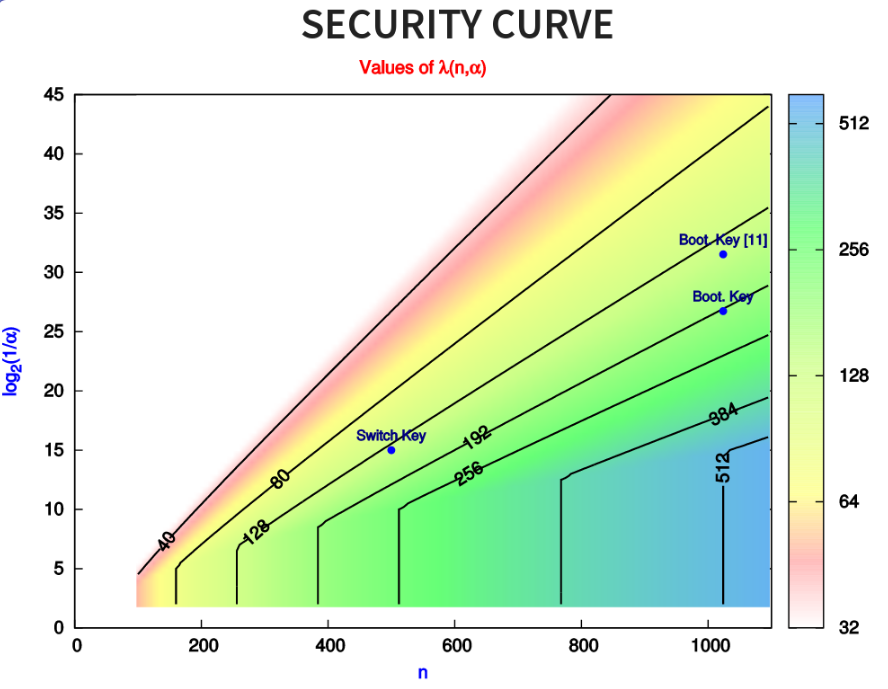
\includegraphics[width=\linewidth]{lambda_tfhe}
    \caption{Curva de seguridad de $\lambda$ (\cite{cheon_faster_2016})}
    \label{fig:lambda_tfhe}
\end{figure}

Tiene una API simple pero muy potente, pero para hacer cualquier cálculo hay que implementarlo desde el nivel más bajo. Los datos cifrados se representan como un array de bits sobre el que se opera como si el dato estuviese en claro. Será este array (codificado en la clase \verb|LweSample|) sobre el que aplicaremos los algoritmos y procedimientos que diseñaremos.

Los elementos de TFHE están codificados en sólo unos pocos grupos:

\begin{itemize}
  \item Parámetros de cifrado (\verb|TFheGateBootstrappingParameterSet|)
  \item Claves
  \begin{itemize}
      \item Privada (\verb|TFheGateBootstrappingSecretKeySet|)
      \item Pública (\verb|TFheGateBootstrappingCloudKeySet|)
  \end{itemize}
  \item Operaciones lógicas sobre texto cifrado (\verb|LweSample|)
  \item Operaciones de cifrado y descifrado
\end{itemize}

Además, TFHE ofrece funciones para limpiar la memoria, dejando en manos del desarrollador la posibilidad de evitar fugas de información una vez no se va a utilizar un elemento.

\subsection{API}

A continuación haremos un repaso de las principales operaciones sobre el texto cifrado incluidas en la librería TFHE.

\begin{itemize}

  \item bootsCONSTANT

  Carga una constante en \verb|value| en la variable cifrada \verb|result|.

  \begin{minted}{c++}
    bootsCONSTANT(LweSample* result, int value,
                  const TFheGateBootstrappingCloudKeySet* bk);
  \end{minted}

  \item bootsNOT

  Niega el valor de la variable \verb|ca| y lo almacena en \verb|result|.

  \begin{minted}{c++}
    bootsNOT(LweSample* result, const LweSample* ca,
             const TFheGateBootstrappingCloudKeySet* bk);
  \end{minted}

  % TODO Alinear y verbatim
  % TODO Etiquetar los códigos
  \item bootsCOPY

  Copia el valor de la variable \verb|ca| y lo almacena en \verb|result|. Cuando se utilizan tanto esta función como las funciones \verb|bootsCONSTANT|  y \verb|bootsNOT| se suele trabajar bit a bit iterando sobre los dos arrays. Si no se hace así, a veces pueden tener comportamientos erráticos.

  \begin{minted}{c++}
    bootsCOPY(LweSample* result, const LweSample* ca,
              const TFheGateBootstrappingCloudKeySet* bk);
  \end{minted}

  \item bootsMUX

  Es una implementación del operador ternario (\verb|a ? b : c|) esencial para poder introducir cómputos con divergencias en su flujo de ejecución aunque (como hemos comentado anteriormente) no podamos modificarlo. Asigna a \verb|result| el valor de \verb|b| si se cumple \verb|a|, si no, le asigna el valor de \verb|c|.

  \begin{minted}{c++}
    bootsMUX(LweSample* result, const LweSample* a,
            const LweSample* b, const LweSample* c,
            const TFheGateBootstrappingCloudKeySet* bk);
  \end{minted}

  Esta función es especialmente interesante, y es la que le da todo el valor a la librería para hacer implementaciones complejas. Por ejemplo, una función con el siguiente código:

  \begin{minted}{c++}
    while (result < 100)
      result = result * 2;
  \end{minted}

  No podría ser implementada sin evaluar el valor de \verb|result|. Sin embargo, con el operador \verb|MUX| podemos hacer lo siguiente (es pseudocódigo):

  \begin{minted}{c++}
    /*
     Hasta que el menor valor que podamos
     escribir con los bits que hemos asignado a
     los decimales (10 bits) no sea mayor que 100
    */
    for (int i = 0.001; i < 100; i = i*2) {
      // es_mayor =  result >= 100
      gte(es_mayor, result, 100);
      // factor = es_mayor ? 2 : 1
      bootsMUX(factor, es_mayor, 2, 1);
      // result = result * factor
      multiplica(result, result, factor);
    }
  \end{minted}

  \item Puertas lógicas

  También implementa las siguientes puertas lógicas booleanas. La utilizaremos como base para hacer el resto de operaciones, como por ejemplo la suma (la función de suma es igual que un circuito sumador).

  \begin{itemize}
    \item \verb|NAND|

    \item \verb|OR|

    \item \verb|AND|

    \item \verb|XOR|

    \item \verb|XNOR|

    \item \verb|NOR|

    \item \verb|ANDNY|, \verb|ANDYN|

    \item \verb|ORNY|, \verb|ORYN|

  \end{itemize}

\end{itemize}

\subsection{Evolución de TFHE}

En su desarrollo se plantea la implementación de un interesante modo conocido como Chimera (\cite{boura_chimera:_2018}) en el que se puedan mover los datos entre el esquema de TFHE y esquemas más eficientes como BFV y CKKS; y viceversa, sin tener que descifrarlos. Esto puede ser útil, por ejemplo, para trabajar con muchas puertas lógicas y hacer alguna operación aritmética rápida entre medias.
